\documentclass[12pt]{article}
\usepackage{xcolor}
\usepackage{amsfonts}
\usepackage{sbc-template}
\usepackage{url,graphicx}
\usepackage[utf8]{inputenc}
\usepackage{amsmath}
\usepackage{comment}
\usepackage[english, brazil]{babel}
\usepackage{indentfirst}
\usepackage{float}
\usepackage{dirtytalk}
\usepackage[ruled,vlined,portuguese]{algorithm2e}
\usepackage{subfigure}
\usepackage[dvips]{epsfig}
\usepackage{algorithmic} 
\usepackage{amsmath}
\usepackage{setspace}
\usepackage{mathtools}
\DeclarePairedDelimiter\ceil{\lceil}{\rceil}
\DeclarePairedDelimiter\floor{\lfloor}{\rfloor}

\sloppy

\title{TEAPS: Triagem Eficiente e Ágil de Pacientes Sintomáticos}

\author{Gustavo Franco Camilo, Lucas Airam Castro de Souza e Vinícius Aguiar Figueiredo}

\address{ Projeto Integrado 2020/2 \\ Universidade Federal do Rio de Janeiro
  (UFRJ)
  }

\date{March 2020}

\begin{document}

\maketitle

\selectlanguage{brazil}


\begin{resumo}
\end{resumo}

\section{Introdução}
\label{sec:introducao}



\section{Proposta}
\label{sec:proposta}

\textcolor{red}{Estrutura em dicionário para traduzir as características de string para número}

\textcolor{red}{Explicar a estrutura dos diretórios}

\begin{figure}[tbh!]
    \centering
    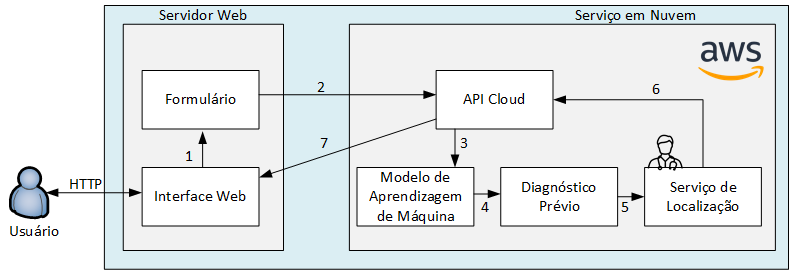
\includegraphics[width=1\textwidth]{figuras/arquitetura.png}
    \caption{\textcolor{red}{Inserir legenda}}
    \label{fig:diagrama-antes}
\end{figure}



\section{Resultados}
\label{sec:resultados}



\nocite{*}

\bibliographystyle{sbc}
\bibliography{references}


\end{document}



